\chapter{Maximum Likelihood Estimation \label{chapter:mlebasics}}

Maximum likelihood (ML) is the most widely used technique for fitting data to probability distributions. In this technique, we choose parameter value(s) for a probability distribution that maximize the probability, or \textbf{likelihood}\index{likelihood}, that it generated our observed data.

\section{Likelihood}

If we draw independent\footnote{Independent sampling just means that the values of different samples do not depend on each other.} samples from the same distribution, $p(x|\theta)$, the {\bf joint density function} for all $n$ observations is:
$$ p(x^{(1)}, x^{(2)}, \dots, x^{(n)}|\theta) = \prod_{i=1}^n p(x^{(i)}|\theta). $$
Since the data are known but the parameter(s) $\theta$ are unknown, we typically view this thing as a function of $\theta$:
$$ \mathcal{L}(\theta) = \prod_{i=1}^n p(x^{(i)}|\theta). $$

The higher the joint probability of the data (the more ``likely'' the data are) given $\theta$, the higher the value of this function. We call $\mathcal{L}(\theta)$ the \textbf{likelihood}\footnote{The distributions we have discussed so far are from a broad family of probability distributions called the {\bf exponential family}. One of the properties of this family is that the log-likelihood is concave. Practically speaking, this means that if we maximize the log-likelihood by setting derivatives equal to zero, we are guaranteed to (a) get only one solution, and (b) find a maximum (not a minimum or an inflection point).}. Frequently we will want to use the logarithm of the likelihood, which we call the \textbf{log-likelihood}, because it has some nice properties, including allowing us to work with sums instead of products\footnote{Note that if the function $f(z)$ has a maximum at $z'$, the function $\log f(z)$ will also have a maximum at $z'$, because the logarithmic function is monotonically increasing. So we will get the same estimate either way.}:
$$ \log \mathcal{L}(\theta) = \sum_{i=1}^n \log p(x^{(i)}|\theta). $$

In {\bf maximum likelihood estimation}\index{maximum likelihood estimation}, we seek to find the $\theta$ for which the likelihood (or log-likelihood) is maximized. We do this by taking derivatives of the log-likelihood with respect to the various parameters and setting them equal to zero. The best-fit parameter estimates obtained in this way are called the \textbf{maximum likelihood estimates (MLEs)}. 

We will now go through a bunch of examples of how to find the MLEs of the probability distributions we saw in Chapter~\ref{chapter:probabilitydistributions}. 

\section{Bernoulli MLE}

First, write down the log-likelihood.
\begin{align*}
\log \mathcal{L}(\mu) &= \sum_{i=1}^n \log p(x^{(i)}|\mu) \\
&= \sum_{i=1}^n \log \left( \mu^{x^{(i)}}(1-\mu)^{1-x^{(i)}} \right) \\
&= \sum_{i=1}^n \left[ x^{(i)} \log(\mu) + (1-x^{(i)}) \log(1-\mu) \right] \end{align*}
Now take the derivative of the log-likelihood with respect to $\mu$:
\begin{align*}
\frac{d}{d \mu} \log \mathcal{L}(\mu) = \sum_{i=1}^n \left[ \frac{x^{(i)}}{\mu} - \frac{1-x^{(i)}}{1-\mu} \right]
\end{align*}
Set this equal to zero and solve for $\hat{\mu}$ (the maximum likelihood estimate of $\mu$):
\begin{align*} \sum_{i=1}^n \left[ \frac{x^{(i)}}{\hat{\mu}} - \frac{1-x^{(i)}}{1-\hat{\mu}} \right] = 0 & \implies (1 - \hat{\mu}) \sum_{i=1}^n x^{(i)} = \hat{\mu} \sum_{i=1}^n (1 - x^{(i)}) \\
& \implies \boxed{\hat{\mu} = \frac{1}{n} \sum_{i=1}^n x^{(i)}} \end{align*}

\section{Binomial MLE}

Here we assume $m$ (the number of trials) is a known quantity. First, write down the log-likelihood.
\begin{align*}
\log \mathcal{L}(\mu) &= \sum_{i=1}^n \log p(x^{(i)}|m,\mu) \\
&= \sum_{i=1}^n \log \left[ {m\choose x} \mu^x (1 - \mu) ^ {m-x} \right] \\
&= \sum_{i=1}^n \left[\log(m!) - \log(x!) - \log((m-x)!) + x^{(i)} \log(\mu) + (m-x^{(i)}) \log(1-\mu) \right] \end{align*}
Now take the derivative of the log-likelihood with respect to $\mu$:
\begin{align*}
\frac{d}{d \mu} \log \mathcal{L}(\mu) = \sum_{i=1}^n \left[ \frac{x^{(i)}}{\mu} - \frac{m-x^{(i)}}{1-\mu} \right]
\end{align*}
Set this equal to zero and solve for $\hat{\mu}$ (the maximum likelihood estimate of $\mu$):
\begin{align*} \sum_{i=1}^n \left[ \frac{x^{(i)}}{\hat{\mu}} - \frac{m-x^{(i)}}{1-\hat{\mu}} \right] = 0 & \implies (1 - \hat{\mu}) \sum_{i=1}^n x^{(i)} = \hat{\mu} \sum_{i=1}^n (m - x^{(i)}) \\
& \implies \boxed{\hat{\mu} = \frac{1}{nm} \sum_{i=1}^n x^{(i)}} \end{align*}

\section{Normal MLE}

First, write down the log-likelihood.
\begin{align*}
\log \mathcal{L}(\mu, \sigma) &= \sum_{i=1}^n \log p(x^{(i)}|\mu, \sigma) \\
&= \sum_{i=1}^n \log \left( \frac{1}{\sqrt{2 \pi \sigma^2}} e^{-\frac{(x^{(i)}-\mu)^2}{2 \sigma^2}} \right) \\
&= -\frac{n}{2} \log (2 \pi) - \frac{n}{2} \log \sigma^2 - \frac{1}{2 \sigma^2} \sum_{i=1}^n \left( x^{(i)} - \mu \right)^2 \\
\end{align*}
To find the MLE for $\mu$, take the derivative of the log-likelihood with respect to $\mu$:
\begin{align*}
\frac{\partial}{\partial \mu} \log \mathcal{L}(\mu, \sigma) = \frac{1}{\sigma^2} \sum_{i=1}^n \left( x^{(i)} - \mu \right)
\end{align*}
Set this equal to zero and solve for $\hat{\mu}$ (the maximum likelihood estimate of $\mu$):
\begin{align*} \frac{1}{\sigma^2} \sum_{i=1}^n \left( x^{(i)} - \mu \right) = 0 & \implies \boxed{\hat{\mu} = \frac{1}{n} \sum_{i=1}^n x^{(i)}} \end{align*}
To find the MLE for $\sigma$, take the derivative of the log-likelihood with respect to $\sigma$:
\begin{align*} \frac{\partial}{\partial \sigma} \log \mathcal{L}(\mu, \sigma) &= -\frac{n}{\sigma} + \frac{1}{\sigma^3} \sum_{i=1}^n \left( x^{(i)} - \mu \right)^2
\end{align*}
Set this equal to zero and solve for $\hat{\sigma}$ (the maximum likelihood estimate of $\sigma$)\footnote{One detail: it turns out this estimate is biased because it depends on the MLE for $\mu$. An unbiased version has $n-1$ in the denominator instead of $n$. The effect of this is minimal unless $n$ is really small.}. Note that the answer depends on our previous MLE of $\mu$:
\begin{align*}
-\frac{n}{\hat{\sigma}} + \frac{1}{\hat{\sigma}^3} \sum_{i=1}^n \left( x^{(i)} - \mu \right)^2 = 0  & \implies \boxed{\hat{\sigma} = \sqrt{\frac{1}{n} \sum_{i=1}^n \left( x^{(i)} - \hat{\mu} \right)^2}}
\end{align*}

\section{Poisson MLE}

First, write down the log-likelihood.
\begin{align*}
\log \mathcal{L}(\lambda) &= \sum_{i=1}^n \log p(x^{(i)}|\lambda) \\
&= \sum_{i=1}^n \log \left( \frac{e^{-\lambda} \lambda^{x^{(i)}}}{x^{(i)}!} \right) \\
&= \sum_{i=1}^n \left[ -\lambda + x^{(i)} \log(\lambda) - \log(x^{(i)}!) \right] \end{align*}
Now take the derivative of the log-likelihood with respect to $\lambda$:
\begin{align*}
\frac{d}{d \lambda} \log \mathcal{L}(\lambda) = \sum_{i=1}^n \left[ -1 + \frac{x^{(i)}}{\lambda} \right]
\end{align*}
Set this equal to zero and solve for $\hat{\lambda}$ (the maximum likelihood estimate of $\lambda$):
\begin{align*} \sum_{i=1}^n \left[ -1 + \frac{x^{(i)}}{\hat{\lambda}} \right] = 0 & \implies \boxed{\hat{\lambda} = \frac{1}{n} \sum_{i=1}^n x^{(i)}} \end{align*}

\section{Geometric MLE}

First, write down the log-likelihood.
\begin{align*}
\log \mathcal{L}(\mu) &= \sum_{i=1}^n \log p(x^{(i)}|\mu) \\
&= \sum_{i=1}^n \log \left( (1-\mu)^{x^{(i)}} \mu \right) \\
&= \sum_{i=1}^n \left[ x^{(i)} \log(1-\mu) + \log(\mu) \right] \end{align*}
Now take the derivative of the log-likelihood with respect to $\mu$:
\begin{align*}
\frac{d}{d \mu} \log \mathcal{L}(\mu) = \sum_{i=1}^n \left[ -\frac{x^{(i)}}{1-\mu} + \frac{1}{\mu} \right]
\end{align*}
Set this equal to zero and solve for $\hat{\mu}$ (the maximum likelihood estimate of $\mu$):
\begin{align*} \sum_{i=1}^n \left[ -\frac{x^{(i)}}{1-\hat{\mu}} + \frac{1}{\hat{\mu}} \right] = 0 & \implies \frac{n}{\hat{\mu}} = \frac{1}{1 - \hat{\mu}} \sum_{i=1}^n x^{(i)} \\
& \implies \boxed{\hat{\mu} = \frac{n}{\sum_{i=1}^n (x^{(i)}+1)} }\end{align*}

\section{Exponential MLE}

First, write down the log-likelihood.
\begin{align*}
\log \mathcal{L}(\lambda) &= \sum_{i=1}^n \log p(x^{(i)}|\lambda) \\
&= \sum_{i=1}^n \log \left( \lambda e^{-\lambda x^{(i)}} \right) \\
&= \sum_{i=1}^n \left[\log(\lambda) - \lambda x^{(i)} \right] \end{align*}
Now take the derivative of the log-likelihood with respect to $\lambda$:
\begin{align*}
\frac{d}{d \lambda} \log \mathcal{L}(\lambda) = \sum_{i=1}^n \left[ \frac{1}{\lambda} - x^{(i)} \right]
\end{align*}
Set this equal to zero and solve for $\hat{\lambda}$ (the maximum likelihood estimate of $\lambda$):
\begin{align*} \sum_{i=1}^n \left[ \frac{1}{\hat{\lambda}} - x^{(i)} \right] = 0 & \implies \boxed{\hat{\lambda} = \frac{n}{\sum_{i=1}^n x^{(i)}}} \end{align*}

\section{Summary}

Why is maximum likelihood estimation useful? When we are fitting a regression model or summarizing some data, we often want to represent that data using a \textbf{model}\index{model}, a simplified representation of the properties of the data and/or how they were generated. A probability distribution is one type of model. Maximum likelihood estimation is one way to go from data to model.

The table below contains a summary of the MLEs of various parameters from different probability distributions.

\begin{center}
\begin{tabular}{lccc}
\toprule
Distribution & Parameter & ML Estimate & Domain of $x^{(i)}$ \\
\midrule
Univariate Normal & $\mu$ & $\displaystyle \cfrac{1}{n} \sum_{i=1}^n x^{(i)}$  & $\mathbb{R}$ \\
& $\sigma$ & $\displaystyle \frac{1}{n} \sum_{i=1}^n \left(x^{(i)} - \hat{\mu}\right)^2 $ & $\mathbb{R}$ \\
Multivariate Normal & $\mu$ & $\displaystyle \frac{1}{n} \sum_{i=1}^n x^{(i)}$ & $\mathbb{R}^m$ \\
& $\boldsymbol\Sigma$ & $\displaystyle \frac{1}{n} \sum_{i=1}^n (x^{(i)}-\hat{\mu})(x^{(i)}-\hat{\mu})^T$ & $\mathbb{R}^m$ \\
Bernoulli & $\mu$ & $\displaystyle \frac{1}{n} \sum_{i=1}^n x^{(i)}$ & $\{0, 1\}$ \\
Binomial (fixed $m$) & $\mu$ & $\displaystyle \frac{1}{nm} \sum_{i=1}^n x^{(i)}$ & $\left\{ 0, 1, \dots, m \right\}$ \\
Poisson & $\lambda$ & $\displaystyle \frac{1}{n} \sum_{i=1}^n x^{(i)}$ & $\left\{ 0, 1, \dots \right\}$\\
Geometric & $\mu$ & $\displaystyle \cfrac{n}{\sum_{i=1}^n (x^{(i)} + 1)} $ & $\left\{ 0, 1, \dots \right\}$ \\
Exponential & $\lambda$ & $\displaystyle \cfrac{n}{\sum_{i=1}^n x^{(i)}} $ & $\mathbb{R}^+$ \\
\bottomrule
\end{tabular}
\end{center}

\section{Discussion Questions}

In Chapter~\ref{chapter:probabilitydistributions}, we examined several examples of experimental conditions and discussed which probability distribution(s) best modeled each one. Here we calculate the maximum likelihood estimates of the parameters of these distributions, based on data.

\begin{enumerate}
\item You are observing several patients' skin in a clinical study to see how long it takes them to develop a rash. You take a picture each day. You observe the following, where $x^{(i)}$ is the number of days of \emph{no rash} before the rash occurs: 

\begin{minipage}[c]{0.5\textwidth}
\begin{center}
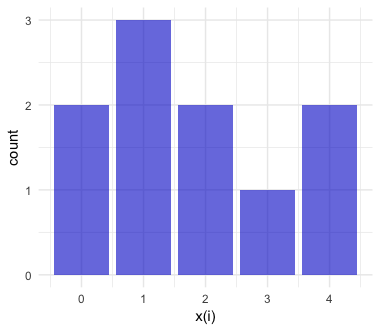
\includegraphics[width=\textwidth]{img/l01-problem2.png}
\end{center}
\end{minipage}
\begin{minipage}[c]{0.5\textwidth}
\begin{center}{\small
\begin{tabular}{cc}
\toprule
Patient ID ($i$) & $x^{(i)}$ \\
\midrule
1 & 4 \\
2 & 1 \\
3 & 0 \\
4 & 2 \\
5 & 2 \\
6 & 4 \\
7 & 3 \\
8 & 1 \\
9 & 0 \\
10 & 1 \\
\end{tabular}}
\end{center}
\end{minipage}
\vspace{3mm}

What distribution should you use to model these data? Calculate the MLE(s) for the parameter(s) of this distribution.
\vspace{3mm}

\item Same situation as above except that instead of taking a picture each day, the patient texts you at the moment he/she observes a rash. The data look like this, where $x^{(i)}$ is the time (in days) at which patient $i$ develops a rash: 

\begin{minipage}[c]{0.5\textwidth}
\begin{center}
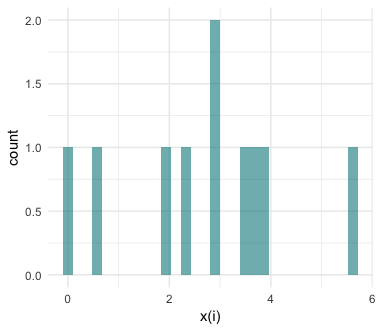
\includegraphics[width=\textwidth]{img/l01-problem3.png}
\end{center}
\end{minipage}
\begin{minipage}[c]{0.5\textwidth}
\begin{center}{\small
\begin{tabular}{cc}
\toprule
Patient ID ($i$) & $x^{(i)}$ \\
\midrule
1 & 2.25 \\
2 & 3.43\\
3 & 0.68\\
4 & 0.04\\
5 & 3.78\\
6 & 5.65\\
7 & 2.88\\
8 & 3.88\\
9 & 2.83\\
10 & 1.87\\
\end{tabular}}
\end{center}
\end{minipage}
\vspace{3mm}

What distribution should you use to model these data? Calculate the MLE(s) for the parameter(s) of this distribution.
\vspace{3mm}

\item Imagine you are Ladislaus Bortkiewicz, and you are modeling the number of persons killed by mule or horse kicks in the Prussian army per year. You have data from the late 1800s over the course of 20 years. Let $x^{(i)}$ be the number of deaths in year $i$.

\begin{minipage}[c]{0.5\textwidth}
\begin{center}
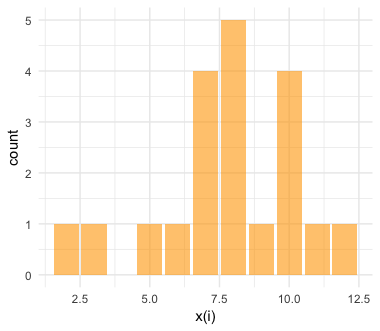
\includegraphics[width=\textwidth]{img/l01-problem4.png}
\end{center}
\end{minipage}
\begin{minipage}[c]{0.5\textwidth}
\begin{center}{\small
\begin{tabular}{cc|cc}
\toprule
Year ($i$) & $x^{(i)}$ & Year ($i$) & $x^{(i)}$ \\
\midrule
1 & 8 & 11 & 9 \\
2 & 10 & 12 & 7 \\
3 & 5 & 13 & 10 \\
4 & 3 & 14 & 12 \\
5 & 10 & 15 & 8 \\
6 & 8 & 16 & 7 \\
7 & 7 & 17 & 8 \\
8 & 2 & 18 & 8 \\
9 & 6 & 19 & 10 \\
10 & 11 & 20 & 7 \\
\end{tabular}}
\end{center}
\end{minipage}
\vspace{3mm}

What distribution should you use to model these data? Calculate the MLE(s) for the parameter(s) of this distribution.
\vspace{3mm}

\item You have waist circumference data on 1045 men aged 70 and above (see Dey's 2002 paper in the Journal of the American Geriatric Society). It looks like this:

\begin{center}
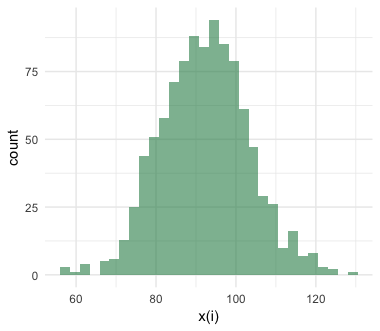
\includegraphics[width=0.5\textwidth]{img/l01-problem5.png}
\end{center}
\vspace{3mm}

What distribution should you use to model these data? Estimate the MLE(s) for the parameter(s) of this distribution.

\end{enumerate}
